% Build from report/: latexmk main.tex
\documentclass[11pt,a4paper]{article}
\usepackage[T1]{fontenc}
\usepackage{lmodern}
\usepackage[margin=23mm]{geometry}
\usepackage{amsmath,amssymb,graphicx,booktabs,tabularx,xcolor}
\usepackage[colorlinks=true,allcolors=blue!55!black,hypertexnames=false]{hyperref}
% Measured values from outputs/double_helix_final, its comparisons and the input diagnostics.
\newcommand{\BlurMinimum}{309}
\newcommand{\BlurMaximum}{1225}
\newcommand{\VerifiedPairs}{133}
\newcommand{\PairCount}{150}
\newcommand{\CandidateTracks}{14,670}
\newcommand{\LongTracks}{3,706}
\newcommand{\MaxTrack}{15}
\newcommand{\FinalRMSE}{0.430}
\newcommand{\FinalPnine}{0.890}
\newcommand{\BeforeBA}{0.485}
\newcommand{\AfterBA}{0.441}
\newcommand{\CenterNear}{0.019\%}
\newcommand{\CenterFar}{5.80\%}
\newcommand{\PointNear}{0.030\%}
\newcommand{\PointFar}{7.55\%}
\newcommand{\RadialK}{-0.01255}
\newcommand{\RibbonCount}{399}
\newcommand{\FullTime}{135.7}
\newcommand{\MatchTime}{86.4}
\newcommand{\ExperimentRows}{%
  Two-view checkpoint & 2/2 & 77 & 0.369 & 792.48 \\
  25 frames, global SIFT & 8/25 & 1,728 & 0.162 & 647.23 \\
  49 frames, 832 px (reference) & 49/49 & 12,609 & 0.226 & 619.24 \\
  49 frames, 1152 px & 49/49 & 12,581 & 0.226 & 619.11 \\
  49 frames, 1536 px & 49/49 & 13,695 & 0.258 & 654.31 \\
  49 frames, 832 px + radial BA & 49/49 & 12,421 & 0.210 & 616.93 \\
}


\begin{document}
\begin{titlepage}
  \centering
  \vspace*{0.24\textheight}
  {\large AI6121 Course Project\par}
  \vspace{1.5em}
  {\LARGE\bfseries Sparse Structure from Motion\\[0.25em] for the NTU Double Helix\par}
  \vspace{0.6em}
  {\large Automatic SIFT correspondence and shared camera self-calibration\par}
  \vspace{3.2em}
  \begin{tabular}{@{}ll@{}}
    \toprule
    \textbf{Name} & \textbf{Matriculation number} \\
    \midrule
    \rule{55mm}{0.35pt} & \rule{47mm}{0.35pt} \\[0.9em]
    \rule{55mm}{0.35pt} & \rule{47mm}{0.35pt} \\[0.9em]
    \rule{55mm}{0.35pt} & \rule{47mm}{0.35pt} \\
    \bottomrule
  \end{tabular}
  \vfill
  {November 2026\par}
\end{titlepage}

\section{Input and objective}

We reconstruct the NTU Double Helix sculpture and its surroundings from a single handheld orbit. The outputs are a colored sparse point cloud and camera poses in a common world frame. The baseline on the manual-projective branch uses the same eight annotated landmarks per image. The experiment here uses automatically matched SIFT features with variable visibility and audits the reconstruction of the metal ribbons separately from the surrounding scene.

The MP4 contains 996 H.264 video frames over 33.16 s. Its coded size is
\(1280\times720\), with a rotation tag that yields \(720\times1280\) working
pixels. We used native display resolution. PyAV reported the encoder
\texttt{Lavf58.20.100} and no usable focal length or lens field in the container
or stream tags. The orbit contact sheet shows continuous viewpoint change,
foreground--background parallax and an overlapping return near the beginning
of the recording. We saw no abrupt cut or field-of-view change in the sampled
frames. The source gives no confirmation of stabilization, rolling-shutter
compensation or dynamic crop. We fit one shared camera model for this segment
and evaluate its sensitivity to initialization. Laplacian variance on the
49 selected grayscale frames ranges from \BlurMinimum\ to \BlurMaximum\
at native resolution. This statistic also responds to texture and is used
as a relative sharpness diagnostic.

\section{Incremental reconstruction}

\paragraph{Observations and camera model.}
Coordinates \((u,v)\) identify work-image pixel centers with origin at the
upper-left pixel center. A resize from display resolution would map
\(u_{\rm work}=s_x(u_{\rm src}+0.5)-0.5\), with the analogous formula for
\(v\). We retain the forward transform and raw working observations. Every
pose follows \(X_c=R_{cw}X_w+t_{cw}\), with camera center
\(C_w=-R_{cw}^{\top}t_{cw}\). For \(X_c=(x,y,z)^\top\), projection is
\[
  q=(x/z,y/z)^\top,\qquad
  \widehat u=c+f\left(1+k_1\|q\|^2\right)q .
\]
The centered principal point \(c=(359.5,639.5)^\top\), zero skew and square
pixels are fixed. The three assumed initial focal lengths are 832, 1152 and
1536 px. The inverse radial model converts raw pixels to normalized rays at
the current \(f,k_1\). Those rays change after BA. Color sampling and pixel
residuals continue to use the original work-image coordinates.

\paragraph{Correspondences and tracks.}
OpenCV detects and describes SIFT keypoints~\cite{lowe2004sift}. The
49-frame balanced configuration uses CLAHE, a lower contrast threshold and
equal feature quotas in 96-pixel grid cells. It compares RootSIFT
descriptors~\cite{arandjelovic2012root}, after L1 normalization and square
root. We apply the nearest-to-second-nearest distance ratio in both
directions and keep mutual correspondences. Temporal neighbors and
end-to-start candidates pass the same verification. Inlier edges are sorted
by geometric error and descriptor distance. A union of two track
components is rejected whenever both components already contain different
features in one image. Track visibility can be incomplete.

\paragraph{Two-view geometry.}
We translate and scale each image's coordinates so the centroid is zero
and the mean radius is \(\sqrt{2}\)~\cite{hartley1997eightpoint}. The
row-major outer products of homogeneous points produce
\(x_b^\top F x_a=0\). SVD gives the right null vector of the eight-point
system. We enforce rank two before undoing the coordinate transforms.
For homogeneous observations the squared Sampson residual is
\[
 d^2 =
 \frac{(x_b^\top F x_a)^2}
 {\|(Fx_a)_{1:2}\|^2+\|(F^\top x_b)_{1:2}\|^2}.
\]
Our RANSAC draws eight distinct pairs, rejects rank-deficient samples,
scores against a 1.5 px threshold and updates the iteration budget from
the inlier proportion. We fit \(F\) in raw pixels at initialization with
\(k_1=0\). This leaves the correspondence graph independent of the focal
hypothesis. Seed generation forms \(K^\top F K\) and uses its singular
vectors to recover the four essential-matrix poses. We refine the
unit-translation direction and rotation using the normalized epipolar
residual. Positive depth, working-pixel reprojection and parallax select a
usable seed. The seed score favors many points with a sufficiently wide
baseline~\cite{hartley2004mvg}.

\paragraph{Map growth.}
DLT triangulation stacks \(q_xP_3-P_1\) and \(q_yP_3-P_2\) for
\(P=[R\mid t]\), takes the least singular vector and divides by its
homogeneous scale. We select and validate a seed ray pair, then try
refitting from consistent observations. The scheduler attempts the frame
with the most existing 3D--2D support first, estimates its pose with
OpenCV PnP RANSAC and refines the inliers. It then adds valid observations
and triangulates new tracks with two or more registered views. This builds
a single reconstruction with one scale~\cite{schonberger2016sfm}. Point
colors are median RGB over active views.

\paragraph{Shared-intrinsics bundle adjustment.}
We minimize Huber loss on each pixel residual component, with a depth
penalty near the camera plane and weak priors on shared intrinsics. The
focal parameter is \(\log f\), with \(f\) bounded to
\([0.45,2]\max(W,H)\) and a prior standard deviation of 0.35 in log
space. The optional radial pass fits \(k_1\) after focal-only optimization,
with bound \(|k_1|\le0.18\), prior standard deviation 0.08 and an
invertibility check at the image corners. The first seed pose is fixed.
One nonzero component of the second seed translation fixes scale.
Distances are in arbitrary units.

The analytical Jacobian connects each observation to its pose, its point
and the shared camera model. We solve damped robust least-squares steps by
eliminating the independent \(3\times3\) point blocks and solving the
reduced camera system with SciPy~\cite{triggs2000bundle}. We reject
steps that fail to decrease robust cost or violate positive depth or
finite projection. We run BA during registration and after map growth.
A final pixel and angle gate updates active observations. Final relative
poses also provide an independent check of the initial pairwise inliers in
the updated normalized camera coordinates.

\section{Verification and experiments}

\paragraph{Ground-truth tests.}
The six deterministic tests cover the eight-point minimal null space,
nonplanar DLT accuracy, planar and pure-rotation degeneracy, and RANSAC
with 20\% incorrect matches. We verify the distorted projection against
OpenCV and the analytical Jacobian against directional finite differences.
A varied-motion synthetic sequence starts at \(f=895\) px and \(k_1=0\)
with truth \(760\) px and \(-0.10\). After focal and radial BA, the test
requires less than 30 px focal error, less than 0.02 radial error and less
than 0.22 px observed reprojection RMSE. An incremental synthetic test
registers six connected views with random missing observations and leaves
a disconnected seventh view visible in the failure records. Camera
centers and 3D points are assessed after similarity alignment.

\paragraph{Video experiments.}
We started with a real two-view pair, then attempted 25 frames sampled
over the whole video. Larger temporal gaps weakened the 3D--2D support
of the 25-frame run. With 49 uniformly spaced frames we retain those 25
source frames and add intermediate views. The balanced 49-frame run
also redistributes features from the highly textured pavement to
lower-contrast regions. Seed 6121 and the frame list are fixed across the
49-frame focal and radial variants.

\begin{table}[htbp]
\centering\small
\begin{tabular}{@{}lrrrr@{}}
\toprule
Run & Registered & Points & Median error (px) & Final \(f\) (px) \\
\midrule
\ExperimentRows
\bottomrule
\end{tabular}
\caption{Actual runs on the Double Helix video. The focal labels describe
working-pixel initialization. Errors are computed from active observations
after final filtering.}
\end{table}

\paragraph{Registration and BA.}
The full orbit verifies \VerifiedPairs\ out of \PairCount\ tested image
pairs and creates \CandidateTracks\ candidate tracks. The final point
cloud has \LongTracks\ tracks with observations in at least three views,
up to \MaxTrack\ views per point. The angular gate is 1 degree and the
final raw-pixel reprojection gate is 3 px. The main run's post-filtering
RMSE is \FinalRMSE\ px, with a 95th percentile of \FinalPnine\ px. On
the fixed observation set of the final focal BA pass, RMSE changes from
\BeforeBA\ to \AfterBA\ px. The final filter and the check after
re-optimization remove 172 points in total. The log retains the
observation counts and costs for both passes.

The weak two-view attempt on source frames 247 and 332 gives 23 mutual
matches and 11 geometric inliers, below the 30-inlier gate. The two-view
checkpoint on 248 and 290 passes the gate. In the 25-frame attempt most
unregistered views lack sufficient correspondences with already
triangulated points despite having edges in the verified match graph.
This illustrates the difference between connected image matches and
connected multiview structure.

\paragraph{Intrinsics and trajectory sensitivity.}
The focal-only starts at 832 and 1152 px yield closely aligned camera
centers and shared 3D points. The 1536 px start gives a larger geometric
difference. After fitting a similarity on the shared camera centers, the
median camera-center differences for the two starts relative to the
832 px run are \CenterNear\ and \CenterFar\ of the reference orbit RMS
radius. The analogous median discrepancies for shared points are
\PointNear\ and \PointFar. The 1536 px run used the full evaluation
budget and its robust cost still decreased. Reprojection medians
alone obscure this sensitivity. The radial experiment gives \(k_1=\RadialK\), improves
the reprojection fit on the same observations, and changes the cloud
and trajectory modestly. We use the simpler focal-only run as the
reference. These are shared-fit estimates, with no measured calibration
or known scene dimensions.

\section{Evidence on the sculpture}

For a separate audit we traced conservative interior regions of the
metal ribbons in the selected images. We excluded the plinth, visible
gaps and uncertain edges. A 3D point qualifies if its measured and
predicted pixels fall inside the eroded regions in at least two active
views. These regions were used only after reconstruction. The 25-frame
trial yielded no confirmed ribbon point under this rule. In the main
49-frame result the audit confirms \RibbonCount\ points. Figure
\ref{fig:ribbon-audit} shows support on the upper loop and lower bands
across multiple views. The coverage is uneven, especially on the dark
smooth side. Several distinct ribbon regions can be seen in the
three-dimensional subset in Figure~\ref{fig:ribbon-cloud}. The points
sample the textured patches and leave large gaps along the ribbons.

\begin{figure}[htbp]
\centering
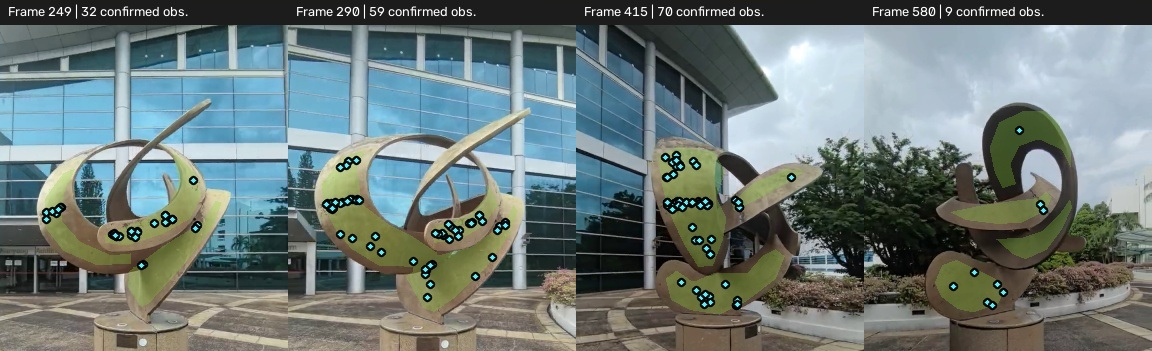
\includegraphics[width=0.96\linewidth]{figures/sfm_ribbon_support.jpg}
\caption{Evaluation regions (green) on four frames, with observations of
audit-confirmed tracks (cyan). The full evidence sheet records every
audited view.}
\label{fig:ribbon-audit}
\end{figure}

\begin{figure}[htbp]
\centering
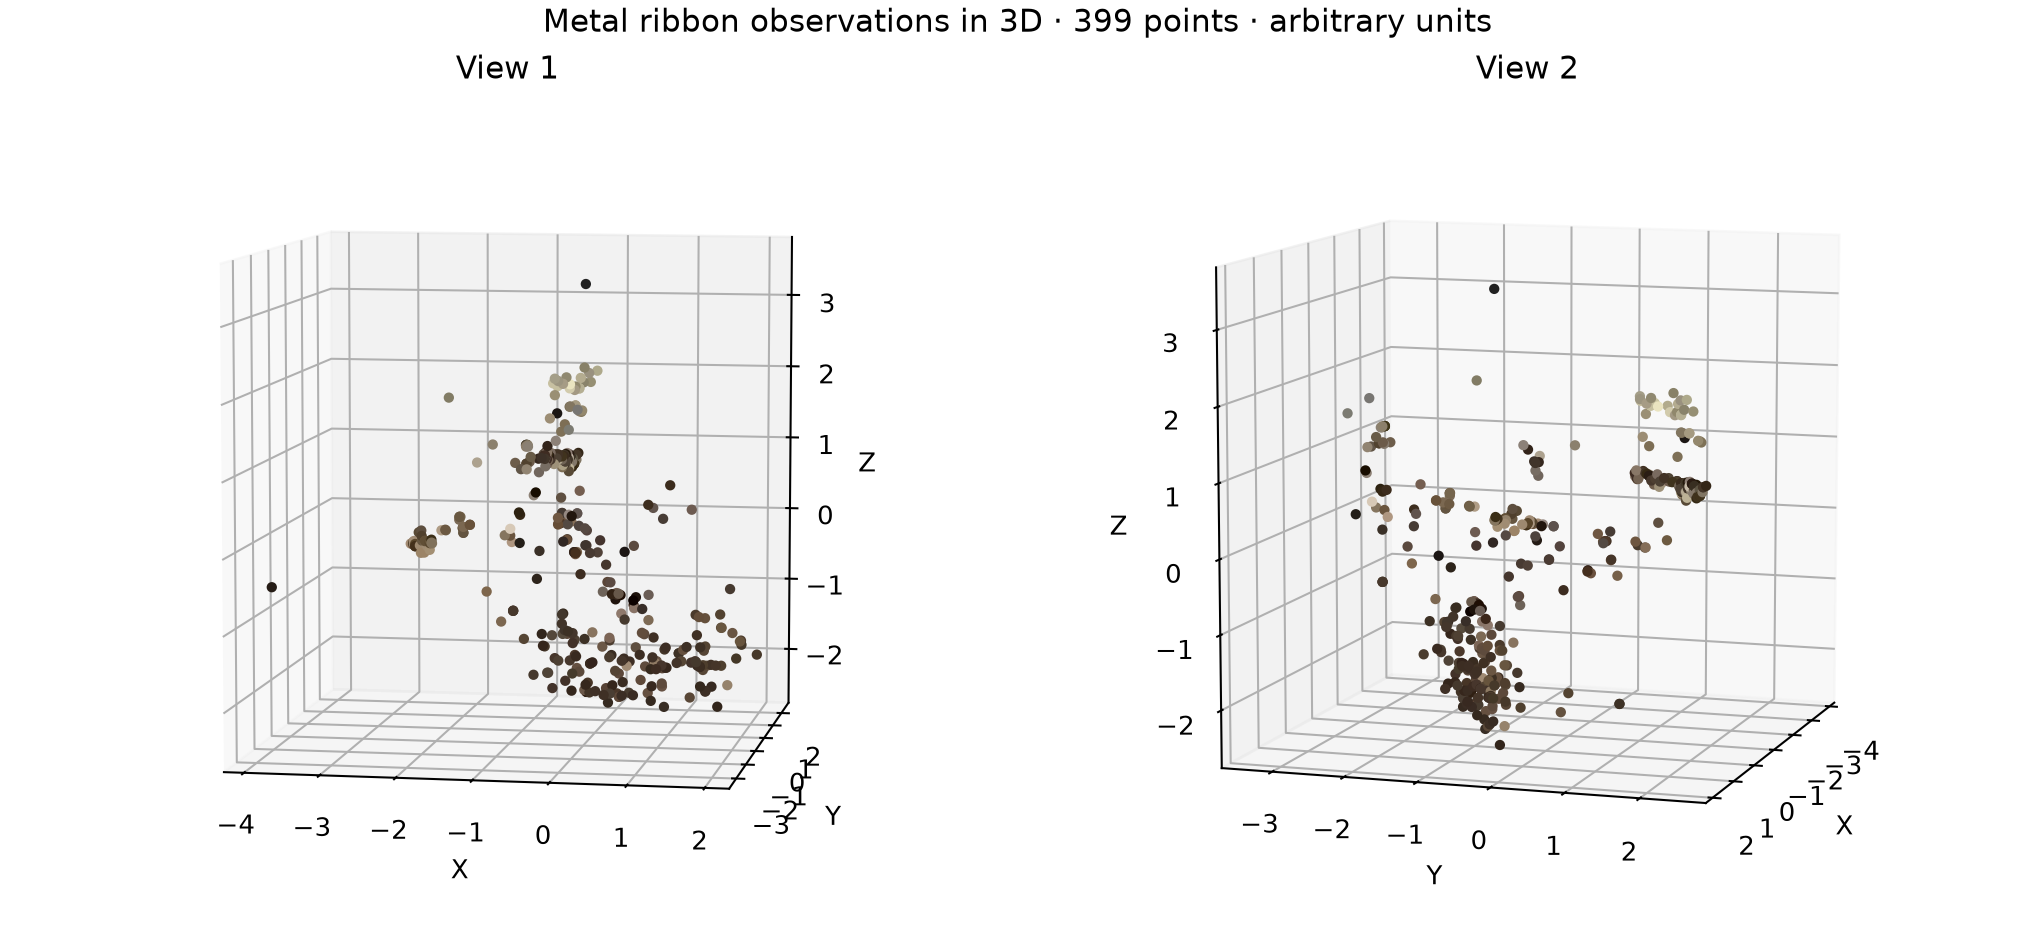
\includegraphics[width=0.98\linewidth]{figures/sfm_ribbon_closeup.png}
\caption{Two viewpoints of the ribbon-supported sparse subset. The plotted
axes are a reorientation of the common world coordinates for display.
Units are arbitrary.}
\label{fig:ribbon-cloud}
\end{figure}

\begin{figure}[htbp]
\centering
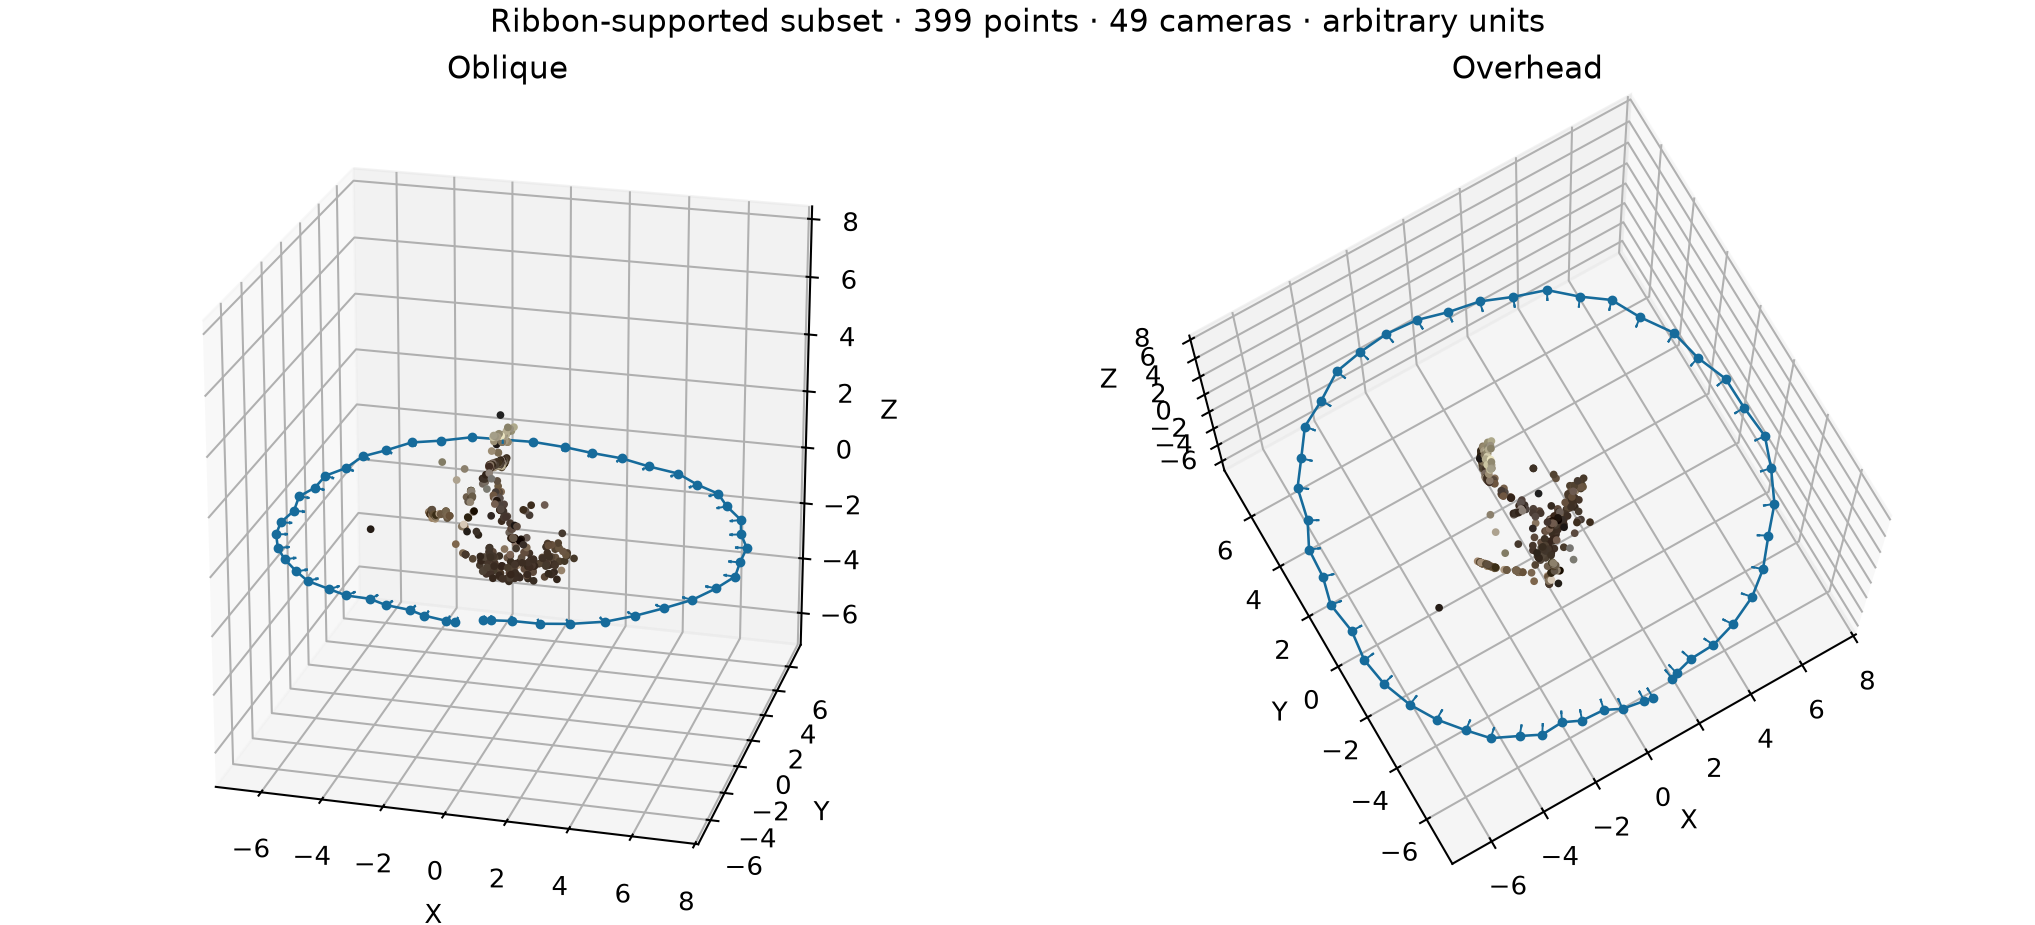
\includegraphics[width=0.95\linewidth]{figures/sfm_ribbon_trajectory.png}
\caption{The same sculpture subset with all registered camera centers and
viewing directions. The full scene PLY also includes pavement and
surrounding structures.}
\end{figure}

\clearpage
\section{Reproduction and limitations}

From the repository root, install the pinned dependencies in
\path{requirements.txt}. The following commands run the synthetic suite
and recreate the main result in a new directory.
\begin{quote}
\small
\begin{verbatim}
python -m unittest discover -s tests -v
python -m sfm reconstruct --video data/video/double_helix.mp4 \
  --config configs/orbit49_balanced.json --output outputs/orbit_repro
python -m sfm.audit outputs/orbit_repro --output outputs/orbit_repro/audit
\end{verbatim}
\end{quote}
The run archives working images, the source-frame mapping,
matches and reprojection plots, per-view status, the configuration and
dependency versions, focal and BA histories, and the colored PLY.
\texttt{python -m sfm.audit} adds the ribbon evidence and PLY.
The corresponding uncached 832 px 49-frame run took \FullTime\ s,
including \MatchTime\ s for matching and geometry verification, on the
CPU run environment. The alternative focal hypotheses reuse the
identical appearance matches.

The full orbit supports a single sparse scene and multiple observed
regions of the metal ribbons. Reliability is limited in smooth and
dark areas. The shared camera assumption can also absorb small
capture-model errors into structure and pose. Additional camera evidence
such as checkerboard images captured in the same recording mode or
reliable original lens and crop information would allow independent
verification of the fitted intrinsics. The current data support an
arbitrary-scale sparse reconstruction.

\section{Software and generative AI disclosure}

OpenCV supplies decoding, image processing, SIFT, descriptor matching,
PnP and Rodrigues conversion. NumPy and SciPy provide numerical
operations and numerical solvers. Matplotlib renders the figures and
PyAV inspects container metadata when ffprobe is unavailable. We implement
the pipeline and geometric stages described above. We used published
methods and library APIs, with no copied third-party SfM code.
OpenAI Codex assisted with the original report template, this
implementation and documentation, synthetic tests and real-data runs,
visual interpretation and drawing the evaluation regions, and report
editing and rendering.

\bibliographystyle{unsrt}
\bibliography{references}
\end{document}
